% Options for packages loaded elsewhere
% Options for packages loaded elsewhere
\PassOptionsToPackage{unicode}{hyperref}
\PassOptionsToPackage{hyphens}{url}
%
\documentclass[
  ignorenonframetext,
]{beamer}
\newif\ifbibliography
\usepackage{pgfpages}
\setbeamertemplate{caption}[numbered]
\setbeamertemplate{caption label separator}{: }
\setbeamercolor{caption name}{fg=normal text.fg}
\beamertemplatenavigationsymbolsempty
% remove section numbering
\setbeamertemplate{part page}{
  \centering
  \begin{beamercolorbox}[sep=16pt,center]{part title}
    \usebeamerfont{part title}\insertpart\par
  \end{beamercolorbox}
}
\setbeamertemplate{section page}{
  \centering
  \begin{beamercolorbox}[sep=12pt,center]{section title}
    \usebeamerfont{section title}\insertsection\par
  \end{beamercolorbox}
}
\setbeamertemplate{subsection page}{
  \centering
  \begin{beamercolorbox}[sep=8pt,center]{subsection title}
    \usebeamerfont{subsection title}\insertsubsection\par
  \end{beamercolorbox}
}
% Prevent slide breaks in the middle of a paragraph
\widowpenalties 1 10000
\raggedbottom
\AtBeginPart{
  \frame{\partpage}
}
\AtBeginSection{
  \ifbibliography
  \else
    \frame{\sectionpage}
  \fi
}
\AtBeginSubsection{
  \frame{\subsectionpage}
}
\usepackage{iftex}
\ifPDFTeX
  \usepackage[T1]{fontenc}
  \usepackage[utf8]{inputenc}
  \usepackage{textcomp} % provide euro and other symbols
\else % if luatex or xetex
  \usepackage{unicode-math} % this also loads fontspec
  \defaultfontfeatures{Scale=MatchLowercase}
  \defaultfontfeatures[\rmfamily]{Ligatures=TeX,Scale=1}
\fi
\usepackage{lmodern}

\usetheme[]{metropolis}
\ifPDFTeX\else
  % xetex/luatex font selection
\fi
% Use upquote if available, for straight quotes in verbatim environments
\IfFileExists{upquote.sty}{\usepackage{upquote}}{}
\IfFileExists{microtype.sty}{% use microtype if available
  \usepackage[]{microtype}
  \UseMicrotypeSet[protrusion]{basicmath} % disable protrusion for tt fonts
}{}
\makeatletter
\@ifundefined{KOMAClassName}{% if non-KOMA class
  \IfFileExists{parskip.sty}{%
    \usepackage{parskip}
  }{% else
    \setlength{\parindent}{0pt}
    \setlength{\parskip}{6pt plus 2pt minus 1pt}}
}{% if KOMA class
  \KOMAoptions{parskip=half}}
\makeatother


\usepackage{longtable,booktabs,array}
\usepackage{calc} % for calculating minipage widths
\usepackage{caption}
% Make caption package work with longtable
\makeatletter
\def\fnum@table{\tablename~\thetable}
\makeatother
\usepackage{graphicx}
\makeatletter
\newsavebox\pandoc@box
\newcommand*\pandocbounded[1]{% scales image to fit in text height/width
  \sbox\pandoc@box{#1}%
  \Gscale@div\@tempa{\textheight}{\dimexpr\ht\pandoc@box+\dp\pandoc@box\relax}%
  \Gscale@div\@tempb{\linewidth}{\wd\pandoc@box}%
  \ifdim\@tempb\p@<\@tempa\p@\let\@tempa\@tempb\fi% select the smaller of both
  \ifdim\@tempa\p@<\p@\scalebox{\@tempa}{\usebox\pandoc@box}%
  \else\usebox{\pandoc@box}%
  \fi%
}
% Set default figure placement to htbp
\def\fps@figure{htbp}
\makeatother

\ifLuaTeX
  \usepackage{luacolor}
  \usepackage[soul]{lua-ul}
\else
  \usepackage{soul}
  \makeatletter
  \let\HL\hl
  \renewcommand\hl{% fix for beamer highlighting
    \let\set@color\beamerorig@set@color
    \let\reset@color\beamerorig@reset@color
    \HL}
  \makeatother
\fi




\setlength{\emergencystretch}{3em} % prevent overfull lines

\providecommand{\tightlist}{%
  \setlength{\itemsep}{0pt}\setlength{\parskip}{0pt}}



 


\setbeamerfont{title}{size=\large} \usepackage{hyperref} \setbeamertemplate{footline}[frame number]
\makeatletter
\@ifpackageloaded{caption}{}{\usepackage{caption}}
\AtBeginDocument{%
\ifdefined\contentsname
  \renewcommand*\contentsname{Table of contents}
\else
  \newcommand\contentsname{Table of contents}
\fi
\ifdefined\listfigurename
  \renewcommand*\listfigurename{List of Figures}
\else
  \newcommand\listfigurename{List of Figures}
\fi
\ifdefined\listtablename
  \renewcommand*\listtablename{List of Tables}
\else
  \newcommand\listtablename{List of Tables}
\fi
\ifdefined\figurename
  \renewcommand*\figurename{Figure}
\else
  \newcommand\figurename{Figure}
\fi
\ifdefined\tablename
  \renewcommand*\tablename{Table}
\else
  \newcommand\tablename{Table}
\fi
}
\@ifpackageloaded{float}{}{\usepackage{float}}
\floatstyle{ruled}
\@ifundefined{c@chapter}{\newfloat{codelisting}{h}{lop}}{\newfloat{codelisting}{h}{lop}[chapter]}
\floatname{codelisting}{Listing}
\newcommand*\listoflistings{\listof{codelisting}{List of Listings}}
\makeatother
\makeatletter
\makeatother
\makeatletter
\@ifpackageloaded{caption}{}{\usepackage{caption}}
\@ifpackageloaded{subcaption}{}{\usepackage{subcaption}}
\makeatother

\usepackage{bookmark}
\IfFileExists{xurl.sty}{\usepackage{xurl}}{} % add URL line breaks if available
\urlstyle{same}
\hypersetup{
  pdfauthor={Giorgio Arcara},
  hidelinks,
  pdfcreator={LaTeX via pandoc}}


\author{Giorgio Arcara}
\date{}

\begin{document}


\begin{frame}
% TITLE SLIDES
\title{Metodi Statistici per la Neuropsicologia Forense\\ \vspace{1em} \emph{1. Introduzione}}
\author{Giorgio Arcara,\\ Università di Padova \\ IRCCS San Camillo, Venezia}

\titlegraphic{

\vspace*{7cm}

\includegraphics[scale=0.15]{Figures/LogoSanCamilloIRCCS_Unipd_alpha.png}
\begin{center}
\vspace{-2.2em}

\includegraphics[scale=0.15]{Figures/CC_license_3_0.png}
\end{center}
}
\date{\today}
\maketitle
\end{frame}

\section{Introduzione}\label{introduzione}

\begin{frame}{Lezione di oggi}
\phantomsection\label{lezione-di-oggi}
\begin{itemize}
\tightlist
\item
  Presentazione del docente e del corso.
\item
  Aspetti organizzativi del corso.
\item
  Obiettivi formativi e ``spirito'' del corso.
\end{itemize}
\end{frame}

\begin{frame}{CV Giorgio Arcara}
\phantomsection\label{cv-giorgio-arcara}
\footnotesize

\begin{itemize}
\item
  Laurea in Psicologia presso Unipd (2005)
\item
  Master in Neuropsicologia dei disturbi cognitivi acquisiti (2006)
\item
  Vari post-doc presso dipartimenti (psicologia, ingegneria,
  neuroscienze)
\item
  Dal 2016 Ricercatore presso IRCCS San Camillo di Venezia.
\item
  Dal 2025 Professore Associato in Psicometria - Università di Padova.
\end{itemize}

\pause

\hfill
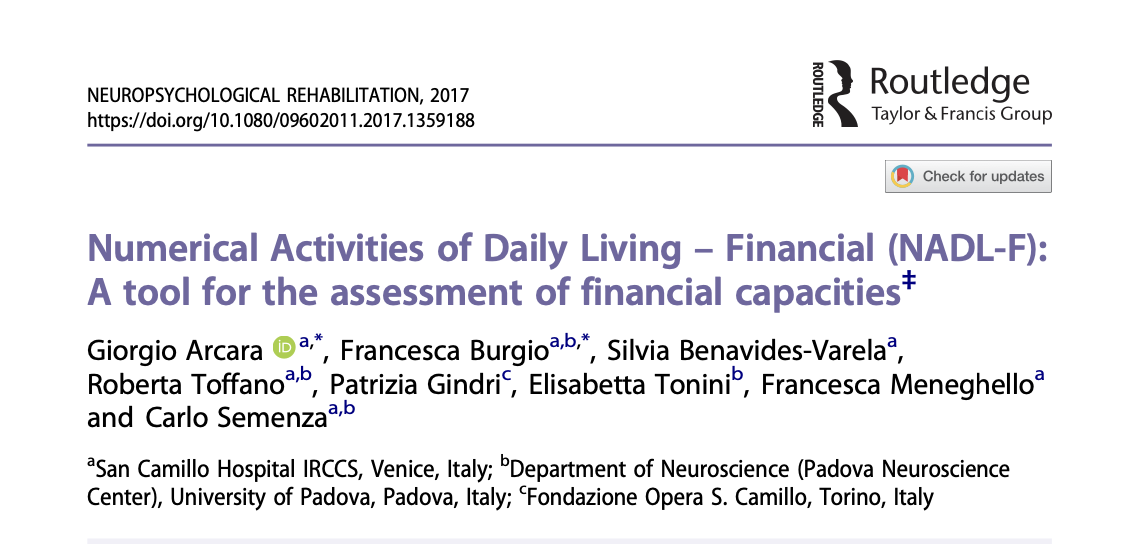
\includegraphics[width=0.6\linewidth,height=\textheight,keepaspectratio]{Figures/NADL_F.png}
\end{frame}

\begin{frame}{Contatti e riferimenti}
\phantomsection\label{contatti-e-riferimenti}
\centering

\href{https://giorgioarcara.github.io}{\ul{https://giorgioarcara.github.io}}

\href{https://www.dpg.unipd.it/category/ruoli/personale-docente?key=4D0707A2DD6FCCD50B90E4C9F316A625}{\ul{pagina
personale unipd}}

\href{mailto:giorgio.arcara@unipd.it}{\nolinkurl{giorgio.arcara@unipd.it}}
\end{frame}

\begin{frame}{Una domanda per iniziare}
\phantomsection\label{una-domanda-per-iniziare}
\begin{center}
Andate su \href{https://www.wooclap.com}{\underline{wooclap.com}} e inserite il codice \textbf{CSEZRQT}

\vspace{1em}

\includegraphics[height=0.6\textheight]{Figures/wooclap_qr_code.png}
\end{center}
\end{frame}

\begin{frame}{Metodi statistici e neuropsicologia forense}
\phantomsection\label{metodi-statistici-e-neuropsicologia-forense}
\begin{center}
\begin{tikzpicture}[
  blocco/.style={draw, thick, rounded corners, fill=gray!10, align=center,
                 text width=4.2cm, minimum height=2.6cm}]

\node[blocco] (ricerca) at (-2.8, 0)
  {Metodi statistici per la \textbf{ricerca} in \mbox{neuropsicologia} forense};
\node[blocco] (valutazione) at (2.8, 0)
  {Metodi statistici per la \textbf{clinica forense} e le \textbf{valutazioni}\\[0.5em]
   \small (consulenze/perizie)};

\draw<2->[red, ultra thick] (valutazione.center) ellipse (3.1cm and 2cm);
\node<2->[text=red, font=\bfseries] at (2.8, -2.4) {Focus di questo corso};

\end{tikzpicture}
\end{center}
\end{frame}

\begin{frame}{Libro di riferimento: \emph{Oltre i punteggi}}
\phantomsection\label{libro-di-riferimento-oltre-i-punteggi}
\begin{columns}
\column{0.45\textwidth}
\begin{center}

\includegraphics[height=0.7\textheight]{Figures/OIP_cover.png}
\end{center}

\column{0.55\textwidth}
\textbf{Oltre i punteggi}\\
\emph{Elementi di psicometria e statistica per la neuropsicologia clinica}

\vspace{1em}
\small
Libro gratuito, in corso di scrittura.

\vspace{1em}
\href{https://giorgioarcara.github.io/oip-book/}{\underline{giorgioarcara.github.io/oip-book}}
\end{columns}
\end{frame}

\begin{frame}{Aspetti organizzativi - Lezioni}
\phantomsection\label{aspetti-organizzativi---lezioni}
\begin{itemize}
\tightlist
\item
  Lezioni online principalmente il mercoledì e il giovedì (dalle 9.00
  alle 11.30 circa). 1 pausa in mezzo.
\item
  Le lezioni saranno videoregistrate e rese disponibile sul moodle.
\item
  Le lezioni prevedono didattica frontale (interattiva) ed esercitazioni
  in classe.
\item
  Saranno trattate poche formule.
\item
  Sono benvenute le domande (in qualsiasi momento).
\item
  Sarà in alcuni casi mostrato del codice in R, ma non è richiesto per
  l'esame.
\end{itemize}
\end{frame}

\begin{frame}{Orari lezioni (dettaglio)}
\phantomsection\label{orari-lezioni-dettaglio}
\scriptsize

\begin{itemize}
\tightlist
\item
  Mercoledì 7 ottobre 2026, 9:00--12:00
\item
  Giovedì 8 ottobre 2026, 9:00--12:00
\item
  Mercoledì 14 ottobre 2026, 9:00--12:00
\item
  Mercoledì 21 ottobre 2026, 9:00--12:00
\item
  Giovedì 22 ottobre 2026, 9:00--12:00
\item
  Mercoledì 4 novembre 2026, 9:00--12:00
\item
  Giovedì 5 novembre 2026, 9:00--12:00
\item
  Venerdì 6 novembre 2026, 9:00-12:00 \_*(lezione che recupera Giovedì
  15)\_
\item
  Mercoledì 11 novembre 2026, 9:00--12:00
\item
  Giovedì 12 novembre 2026, 9:00--12:00
\item
  Mercoledì 18 novembre 2026, 9:00--12:00
\item
  Giovedì 19 novembre 2026, 9:00--12:00
\item
  Mercoledì 25 novembre 2026, 9:00--12:00
\item
  Giovedì 26 novembre 2026, 9:00--12:00
\end{itemize}
\end{frame}

\begin{frame}{Aspetti organizzativi - Materiali}
\phantomsection\label{aspetti-organizzativi---materiali}
\textbf{Condividerò tutto il materiale utilizzato e mostrato}

I materiali principali sono le slides e materiali aggiuntivi che vi saranno forniti durante il corso. I materiali li troverete anche a questo link \href{https://github.com/giorgioarcara/Slides-Metodi-Statistici-Neuropsi-Forense}{\underline{github}}

Condividerò anche script di R e sarà dato risalto a ``simulazioni'' di
dati per comprensione dei concetti, con script sviluppati durante il
corso (utili, non necessari).
\end{frame}

\begin{frame}{Aspetti organizzativi - Slides e handouts}
\phantomsection\label{aspetti-organizzativi---slides-e-handouts}
Il materiale del corso è costituito da:

\begin{itemize}
\tightlist
\item
  \textbf{slides} delle lezioni;
\item
  \textbf{handouts} (dispense di approfondimento) su argomenti
  specifici, se ritenuti necessari.
\end{itemize}
\end{frame}

\begin{frame}{Aspetti organizzativi - Materiali}
\phantomsection\label{aspetti-organizzativi---materiali-1}
\begin{columns}
\column{0.5\textwidth}
\small
\emph{Mondini, S., Cappelletti, M., \& Arcara, G. (2022). Methodology in Neuropsychological Assessment: An Interpretative Approach to Guide Clinical Practice. Taylor \& Francis.}\\
\vspace{1em}
Testo di approfondimento, \textbf{non indispensabile}.

\column{0.5\textwidth}

\begin{figure}
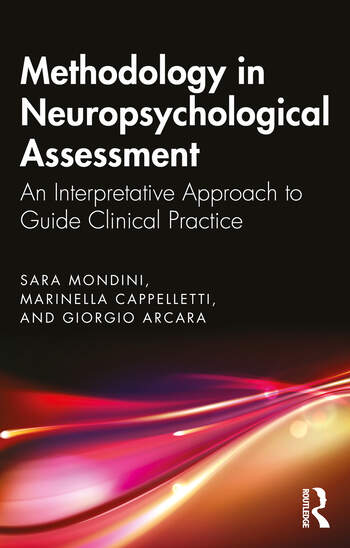
\includegraphics[scale=0.5]{Figures/Methodology_book.png}
\end{figure}

\end{columns}
\end{frame}

\begin{frame}{Aspetti organizzativi - Materiali aggiuntivi}
\phantomsection\label{aspetti-organizzativi---materiali-aggiuntivi}
\begin{itemize}
\item
  Libro gratuito su statistica base ed R
  \href{https://learningstatisticswithr.com/}{\underline{https://learningstatisticswithr.com/}}
\item
  Libro gratuito su psicometria (più avanzato)
  \href{https://personality-project.org/r/book/}{\underline{https://personality-project.org/r/book/}}
\item
  \emph{Oltre i punteggi} (libro in corso di scrittura)
  \href{https://giorgioarcara.github.io/oip-book/}{\underline{https://giorgioarcara.github.io/oip-book/}}
\end{itemize}
\end{frame}

\begin{frame}{Aspetti organizzativi - Moodle}
\phantomsection\label{aspetti-organizzativi---moodle}
Il Moodle del corso è organizzato in due parti separate:

\begin{itemize}
\tightlist
\item
  una sezione con le \textbf{lezioni} (registrazioni e materiali di ogni
  lezione);
\item
  una sezione con gli \textbf{argomenti} del corso.
\end{itemize}

\vspace{1em}

La corrispondenza tra lezioni e argomenti non è fissa: dipende da
interazioni e domande che possono emergere durante la lezione.
\end{frame}

\begin{frame}{Aspetti organizzativi - Esami}
\phantomsection\label{aspetti-organizzativi---esami}
Gli esami saranno scritti con:

\begin{itemize}
\tightlist
\item
  4 domande aperte su aspetti teorici.
\item
  domande su scenari applicativi in cui ragionare per applicare le
  conoscenze sviluppate.
\end{itemize}

Gli esami saranno poco nozionistici e più di ragionamento

\underline{Non sarà necessario ricordare a memoria nessuna formula}
\end{frame}

\begin{frame}{Stile di insegnamento}
\phantomsection\label{stile-di-insegnamento}
\begin{center}
\begin{tikzpicture}
% piramide della Tassonomia di Bloom (dal basso verso l'alto)
\foreach \i/\lab/\c/\t in {0/Ricordare/15/black, 1/Comprendere/30/black, 2/Applicare/45/black,
                           3/Analizzare/60/white, 4/Valutare/75/white, 5/Creare/90/white} {
  \pgfmathsetmacro{\ya}{\i*0.9}
  \pgfmathsetmacro{\yb}{(\i+1)*0.9}
  \pgfmathsetmacro{\ym}{(\i+0.5)*0.9}
  \pgfmathsetmacro{\wa}{4.5*(1-\ya/6.6)}
  \pgfmathsetmacro{\wb}{4.5*(1-\yb/6.6)}
  \fill[mDarkTeal!\c!white, draw=white, line width=1.5pt]
    (-\wa,\ya) -- (\wa,\ya) -- (\wb,\yb) -- (-\wb,\yb) -- cycle;
  \node[text=\t, font=\small\bfseries] at (0,\ym) {\lab};
}
\node[font=\scriptsize] at (0,-0.45) {Tassonomia di Bloom (rivista; Anderson \& Krathwohl, 2001)};
\end{tikzpicture}
\end{center}
\end{frame}

\begin{frame}{Utilizzo critico di LLM (es. ChatGPT) per il corso 1/2}
\phantomsection\label{utilizzo-critico-di-llm-es.-chatgpt-per-il-corso-12}
I Large Language Models (LLM) come ChatGPT, comunemente chiamati sistemi
di intelligenza artificiale sono una grande opportunità di innovazione
tecnologica che merita di essere discussa. Di seguito alcune
raccomandazioni per un utilizzo appropriato per il corso.
\end{frame}

\begin{frame}{Utilizzo critico di LLM (es. ChatGPT) per il corso 2/2}
\phantomsection\label{utilizzo-critico-di-llm-es.-chatgpt-per-il-corso-22}
\begin{itemize}
\item
  Non cercate risposte, ma cercate \emph{una guida} per trovare
  informazioni. Gli LLM funzionano come motori di ricerca avanzati
  soprattutto se la domanda è vaga.
\item
  Utilizzatele per capire meglio alcuni concetti. Se qualcosa non è
  chiaro, potete esplicitamente chiedere di spiegarlo in altri termini o
  con altri esempi.
\item
  \textbf{Non vi fidate ciecamente di ciò che dicono} ma cercate
  conferma da eventuali fonti. Gli LLM spesso mostrano dei comportamenti
  detti \emph{hallucinations}, che danno risposte verosimili o credibili
  ma che si rivelano sbagliate o completamente inventate.
\end{itemize}
\end{frame}

\begin{frame}{Neuropsicologia Forense}
\phantomsection\label{neuropsicologia-forense}
\begin{center}
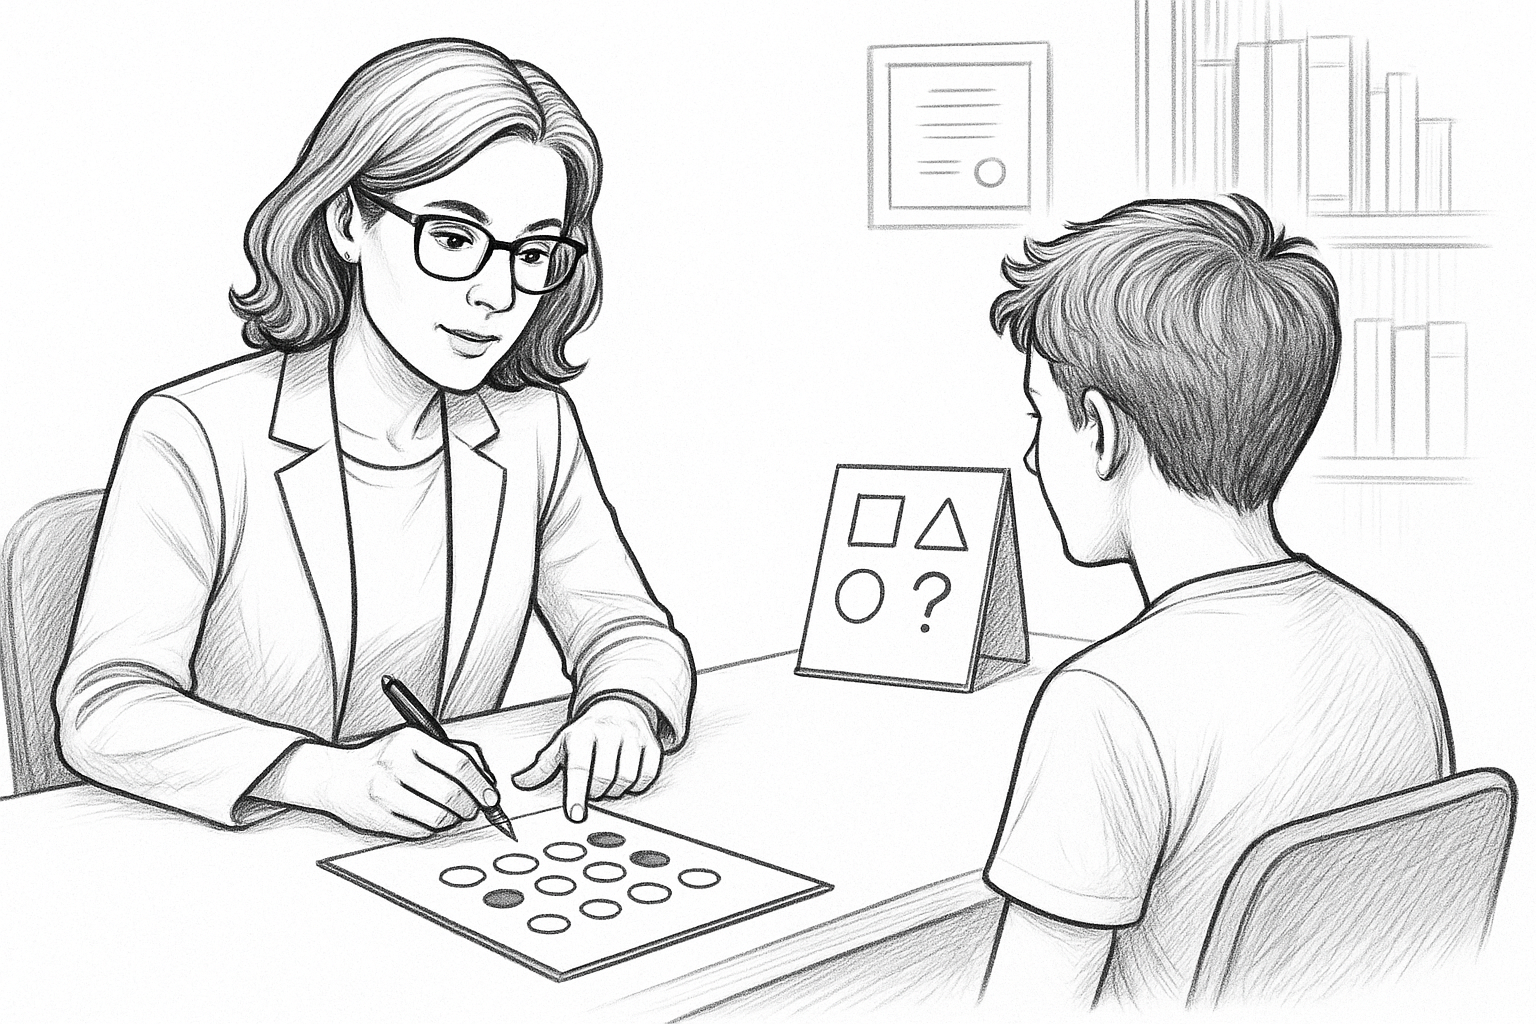
\includegraphics[width=0.5\linewidth,height=\textheight,keepaspectratio]{Figures/Valutazione_Neuropsi_ChatGPT.png}
\end{center}
\pause

\textbf{Valutazione neuropsicologica}: esame clinico per indagare il
funzionamento cognitivo a fine descrittivo o diagnostico. In genere sono
somministrati una serie di \emph{test neuropsicologici} ad un individuo
per indagare il suo funzionamento cognitivo.

Sono ottenuti punteggi e questi sono confrontati con valori di
riferimento per trarre conclusioni (es. è presente un deficit
cognitivo.)
\end{frame}

\begin{frame}{Neuropsicologia Forense}
\phantomsection\label{neuropsicologia-forense-1}
Dietro la semplicità di quanto descritto ci sono tanti aspetti
metodologici (psicometrici e statistici) che saranno approfonditi in
questo corso.
\end{frame}

\begin{frame}{Obiettivi del corso}
\phantomsection\label{obiettivi-del-corso}
Partiamo dalla fine:

\begin{itemize}
\tightlist
\item
  Fornire elementi di conoscenza statistica e ragionamento critico utili
  per la neuropsicologia forense
\item
  Fornire conoscenze sia per la pratica di psicologia forense, sia per
  chi vuole fare ricerca in ambito forense.
\item
  Fornire conoscenze sull'elemento cardine per la valutazione forense:
  il test cognitivo o neuropsicologico, con le sue potenzialità e
  limiti.
\item
  Fornire conoscenze base su test statistici applicati al caso singolo.
\end{itemize}

\pause

\emph{Obiettivo bonus}: superare alcuni traumi che vi ha dato la
statistica a Psicologia
\end{frame}

\begin{frame}{Attività: perché la statistica è utile per il
neuropsicologo forense?}
\phantomsection\label{attivituxe0-perchuxe9-la-statistica-uxe8-utile-per-il-neuropsicologo-forense}
\begin{center}

\includegraphics[height=0.65\textheight]{Figures/padlet_qr_code.png}
\end{center}
\end{frame}

\begin{frame}{Perché è utile la statistica per il neuropsicologo
forense? (1/2)}
\phantomsection\label{perchuxe9-uxe8-utile-la-statistica-per-il-neuropsicologo-forense-12}
\begin{columns}
\column{0.5\textwidth}

\begin{figure}
\includegraphics[width=0.8\textwidth]{Figures/Motore.png}
\end{figure}
\tiny{Non serve conoscere come funziona un motore per guidare una macchina. Basta sapere cosa è giusto o sbagliato fare con pedali, cambio e volante. (Aforisma di H. Baayen, corso di statistica, Edmonton 2008 circa)}

\pause
\column{0.5\textwidth}

\begin{figure}
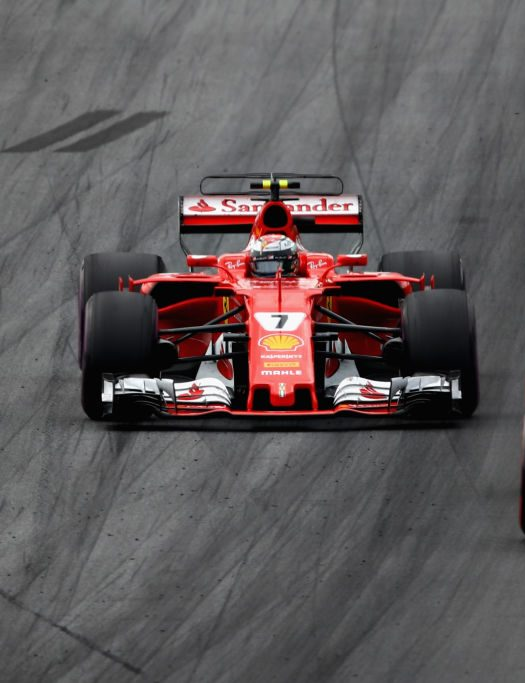
\includegraphics[width=0.8\textwidth]{Figures/F1.png}
\end{figure}
\tiny{I piloti di formula 1 hanno conoscenze superiori su come funziona un motore.}

\end{columns}
\end{frame}

\begin{frame}{Perché è utile la statistica per il neuropsicologo
forense? (2/2)}
\phantomsection\label{perchuxe9-uxe8-utile-la-statistica-per-il-neuropsicologo-forense-22}
\begin{columns}
\column{0.5\textwidth}

\begin{figure}

\includegraphics[width=0.7\textwidth]{Figures/Mechanic_ChatGPT_BN.png}
\end{figure}
\tiny{Un pilota di F1 non è però un ingegnere o un meccanico: ne conosce bene il funzionamento per accorgersi di problemi (es. vibrazioni o rumori insoliti) e comunicare con il team, ma resta un utilizzatore, che deve concentrarsi sulle proprie abilità di guida.}

\column{0.5\textwidth}
Lo stesso vale per la/il neuropsicologa/o: non è necessario essere "psicometriste/i" o "statiste/i" per usare bene i test, ma conoscerne meglio il funzionamento aiuta a notare possibili problemi e a sfruttarne meglio le potenzialità.
\end{columns}
\end{frame}

\begin{frame}{5 principi basilari di questo corso (1)}
\phantomsection\label{principi-basilari-di-questo-corso-1}
\begin{enumerate}
\tightlist
\item
  la valutazione neuropsicologica forense è innanzitutto una valutazione
  clinica
\end{enumerate}

\vspace{3em}

\emph{Per una buona perizia/consulenza, bisogna avere competenze
cliniche (in particolare sono rilevanti le capacità diagnostiche)}
\end{frame}

\begin{frame}{5 principi basilari di questo corso (2)}
\phantomsection\label{principi-basilari-di-questo-corso-2}
\begin{enumerate}
\setcounter{enumi}{1}
\tightlist
\item
  In questo corso di Laurea (non solo nelle mie lezioni) il leitmotiv
  sarà che nella valutazione forense hanno un ruolo fondamentale le
  valutazioni di tipo cognitivo.
\end{enumerate}

\vspace{3em}

\emph{Un approccio che si sta imponendo in ambito forense è quello di
sostanziare in maniera il più obiettiva/oggettiva possibile le vostre
argomentazioni.}

\emph{Questo si contrappone ad un approccio dominante alla valutazione
forense come semplice giudizio clinico, magari da fonte autorevole, o i
test proiettivi, etc.}
\end{frame}

\begin{frame}{5 principi basilari di questo corso (3)}
\phantomsection\label{principi-basilari-di-questo-corso-3}
\begin{enumerate}
\setcounter{enumi}{2}
\tightlist
\item
  la valutazione neuropsicologica non è solo somministrazione di test ma
  raccolta di evidenze e stesura di una relazione.
\end{enumerate}

\vspace{3em}

\emph{Il concetto di raccolta di evidenze sarà un tema ricorrente di
questo corso e gli aspetti statistici saranno presentati come alcune
delle possibili evidenze.}
\end{frame}

\begin{frame}{5 principi basilari di questo corso (4)}
\phantomsection\label{principi-basilari-di-questo-corso-4}
\begin{enumerate}
\setcounter{enumi}{3}
\tightlist
\item
  Rispetto alla valutazione neuropsicologica puramente clinica, nella
  valutazione forense ci sono possibili problemi aggiuntivi (es.
  simulazione). \vspace{3em}
\end{enumerate}

\emph{Non è richiesta solo competenza clinica, ma anche competenze
aggiuntive specifiche per valutazione forense.}
\end{frame}

\begin{frame}{5 principi basilari di questo corso (5)}
\phantomsection\label{principi-basilari-di-questo-corso-5}
\begin{enumerate}
\setcounter{enumi}{4}
\tightlist
\item
  In molti casi di forense (es. consulenze tecniche/perizie), a dispetto
  della valutazione neuropsicologica puramente clinica, è possibile che
  ci sia anche un'altra parte che farà un'altra valutazione e relazione,
  e l'obiettivo è anche creare una relazione più convincente (su basi
  argomentative e oggettive) dell'altra parte. \vspace{2em}
\end{enumerate}

\pause
\begin{figure}
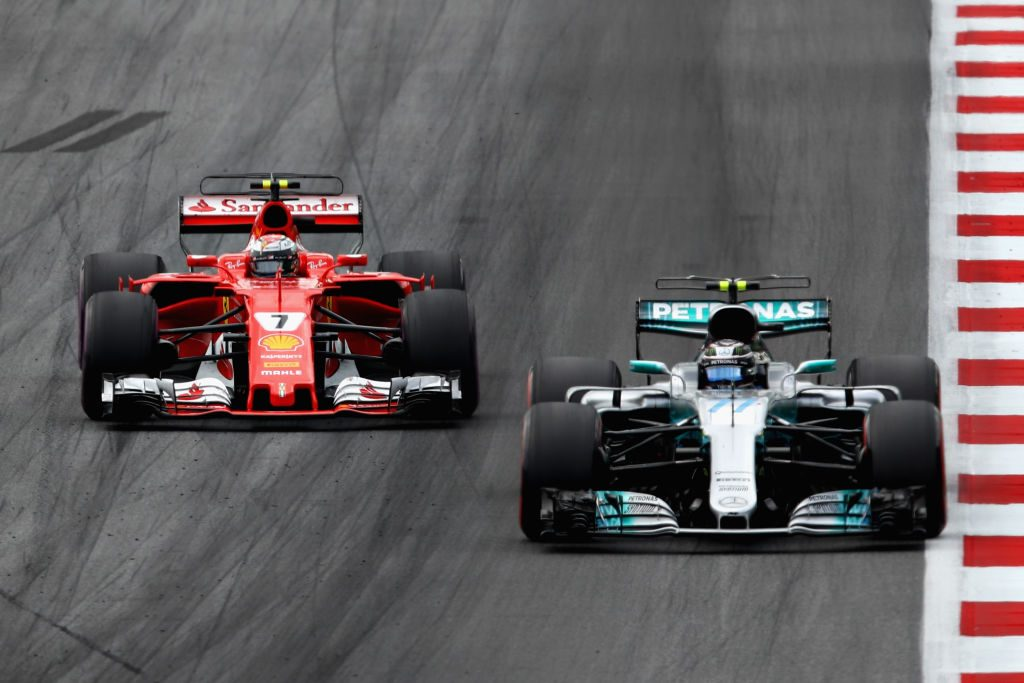
\includegraphics[width=0.4\textwidth]{Figures/F1_2.jpg}
\end{figure}
\end{frame}

\begin{frame}{Alcune domande a cui risponderete}
\phantomsection\label{alcune-domande-a-cui-risponderete}
\emph{Come posso dimostrare che i test utilizzati per la mia perizia
sono migliori di quelli dell'altra parte?} \pause \emph{Come posso
dimostrare che nell'interpretare i test, l'altra parte ha commesso un
errore?}
\end{frame}

\begin{frame}{Focus sui test neuropsicologici}
\phantomsection\label{focus-sui-test-neuropsicologici}
Anche se la metodologia della valutazione neuropsicologica forense in
genere include vari aspetti, Il focus sulla lezione è sui test
neuropsicologici, su cosa sono, come si creano, come si interpretano i
risultati.

Questo perché l'utilizzo dei test rappresenta una fase fondamentale
della valutazione neuropsicologica.

\pause

(altre fasi che non sono trattate sono l'intervista, il colloquio con i
familiari, anche se sarà accennato il perché della loro rilevanza.)
\end{frame}

\begin{frame}{Focus sui test statistici per caso singolo}
\phantomsection\label{focus-sui-test-statistici-per-caso-singolo}
Il più delle volte in ambito forense, l'interesse è dare delle risposte
su un singolo individuo.

Da un punto di vista statistico questo significa utilizzare metodi che
permettono di rispondere non a campioni, ma a singoli individui (ed è
qualcosa di particolarmente rilevante)
\end{frame}

\begin{frame}{Attività: perché si usano i test in neuropsicologia
forense?}
\phantomsection\label{attivituxe0-perchuxe9-si-usano-i-test-in-neuropsicologia-forense}
\begin{center}

\includegraphics[height=0.65\textheight]{Figures/padlet_qr_code.png}
\end{center}
\end{frame}

\begin{frame}{Ruolo dei test}
\phantomsection\label{ruolo-dei-test}
\emph{Perché si utilizzano i test in neuropsicologia clinica e in
neuropsicologia forense?}

\pause

Per ottenere informazioni rilevanti alla fine degli scopi della
valutazione e per superare i limiti di una valutazione soggettiva basata
solo su giudizi clinici.
\end{frame}

\begin{frame}{Perché non fornire direttamente la lista dei test
migliori?}
\phantomsection\label{perchuxe9-non-fornire-direttamente-la-lista-dei-test-migliori}
I test esistenti in neuropsicologia clinica sono innumervoli
(centinaia). Ogni elenco sarebbe parziale.

Il loro utilizzo dipende anche dalle circostanze e dalla domanda per cui
viene effettuata la valutazione.

I test moderni (e migliori) oggi, saranno potenzialmente superati l'anno
prossimo.
\end{frame}

\begin{frame}{Scegliere i test}
\phantomsection\label{scegliere-i-test}
\setlength{\fboxrule}{1mm}
\fcolorbox{red}{white}{\rule{0pt}{12pt}\hspace{2pt} Alcuni test sono meglio degli altri\hspace{2pt}}, ma la scelta dei test dipende anche  dalle circostanze: dal motivo della valutazione, dal contesto clinico, dalla patologia trattata, dal tempo a disposizione, dalle risorse economiche a disposizione, dai gusti del
neuropsicologo, etc.
\end{frame}

\begin{frame}{Statistica e Psicometria}
\phantomsection\label{statistica-e-psicometria}
La \textbf{statistica} è quella disciplina che si occupa di come
possiamo trarre delle conclusione a partire da dati empirici e si occupa
di ogni fase (pianificazione, raccolta, analisi, interpretazione).
\pause

La \textbf{psicometria} è quella disciplina che si occupa di misurazione
in psicologia e di inferenze statistiche di concetti psicologici.
\end{frame}

\begin{frame}{Perché sono importanti psicometria e statistica?}
\phantomsection\label{perchuxe9-sono-importanti-psicometria-e-statistica}
Non basta che un test sia ``pubblicato'' o ``validato'' perché sia
utilizzabile senza una riflessione critica.

\vspace{2em}

Grazie alle conoscenze metodologiche possiamo scegliere quale test è
meglio di un altro.

\pause
\vspace{2em}

\begin{center}
\begin{tikzpicture}[baseline=(current bounding box.center)]

% Prima riga: sbagliato - giusto
\node[anchor=west] at (0, 0) {\textbf{Sbagliato}};
\node[anchor=east] at (10, 0) {\textbf{Giusto}};
\draw[thick] (1.8, 0) -- (8.5, 0);

% X al centro
\node[text=red, font=\bfseries\Huge] at (5, 0) {X};

% Seconda riga: peggio - meglio
\node[anchor=west] at (0, -1.2) {\textbf{Peggio}};
\node[anchor=east] at (10, -1.2) {\textbf{Meglio}};
\draw[thick] (1.5, -1.2) -- (8.5, -1.2);

\end{tikzpicture}
\end{center}
\end{frame}

\begin{frame}{Perché psicometria/statistica a volte sono tralasciati?
(1/3)}
\phantomsection\label{perchuxe9-psicometriastatistica-a-volte-sono-tralasciati-13}
\begin{itemize}
\tightlist
\item
  Le abilità cliniche/forensi trascendono le conoscenze
  metodologiche/psicometriche. \emph{si può essere ottimi neuropsicologi
  clinici/forensi senza conoscere questi aspetti}
\end{itemize}
\end{frame}

\begin{frame}{Perché psicometria/statistica a volte sono tralasciati?
(2/3)}
\phantomsection\label{perchuxe9-psicometriastatistica-a-volte-sono-tralasciati-23}
\begin{itemize}
\tightlist
\item
  In neuropsicologia clinica non ci sono feedback chiari di un utilizzo
  inadeguato dei test.
\end{itemize}

\emph{(cosa succede se sbaglio clamorosamente nell'interpretazione di un
test? Non molto)}
\end{frame}

\begin{frame}{Perché psicometria/statistica a volte sono tralasciati?
(3/3)}
\phantomsection\label{perchuxe9-psicometriastatistica-a-volte-sono-tralasciati-33}
\begin{itemize}
\tightlist
\item
  È più facile fidarsi ``ciecamente'' di un test, e delegare la
  responsabilità al test (invece che prendersela come neuropsicologi) ed
  è più semplice considerarlo come uno strumento oggettivo.
\end{itemize}

\emph{(è stato il test a dirlo, non io!)}
\end{frame}

\begin{frame}{La situazione attuale}
\phantomsection\label{la-situazione-attuale}
In neuropsicologia forense non c'è (ad oggi) una forte cultura
psicometrica e statistica. Molti di questi limiti derivano direttamente
dalla neuropsicologia clinica.

Ci sono numerose pratiche problematiche (es. uso non consapevole dei
punti-z)
\end{frame}

\begin{frame}{Valutazione neuropsicologica come raccolta di
informazioni}
\phantomsection\label{valutazione-neuropsicologica-come-raccolta-di-informazioni}
\pandocbounded{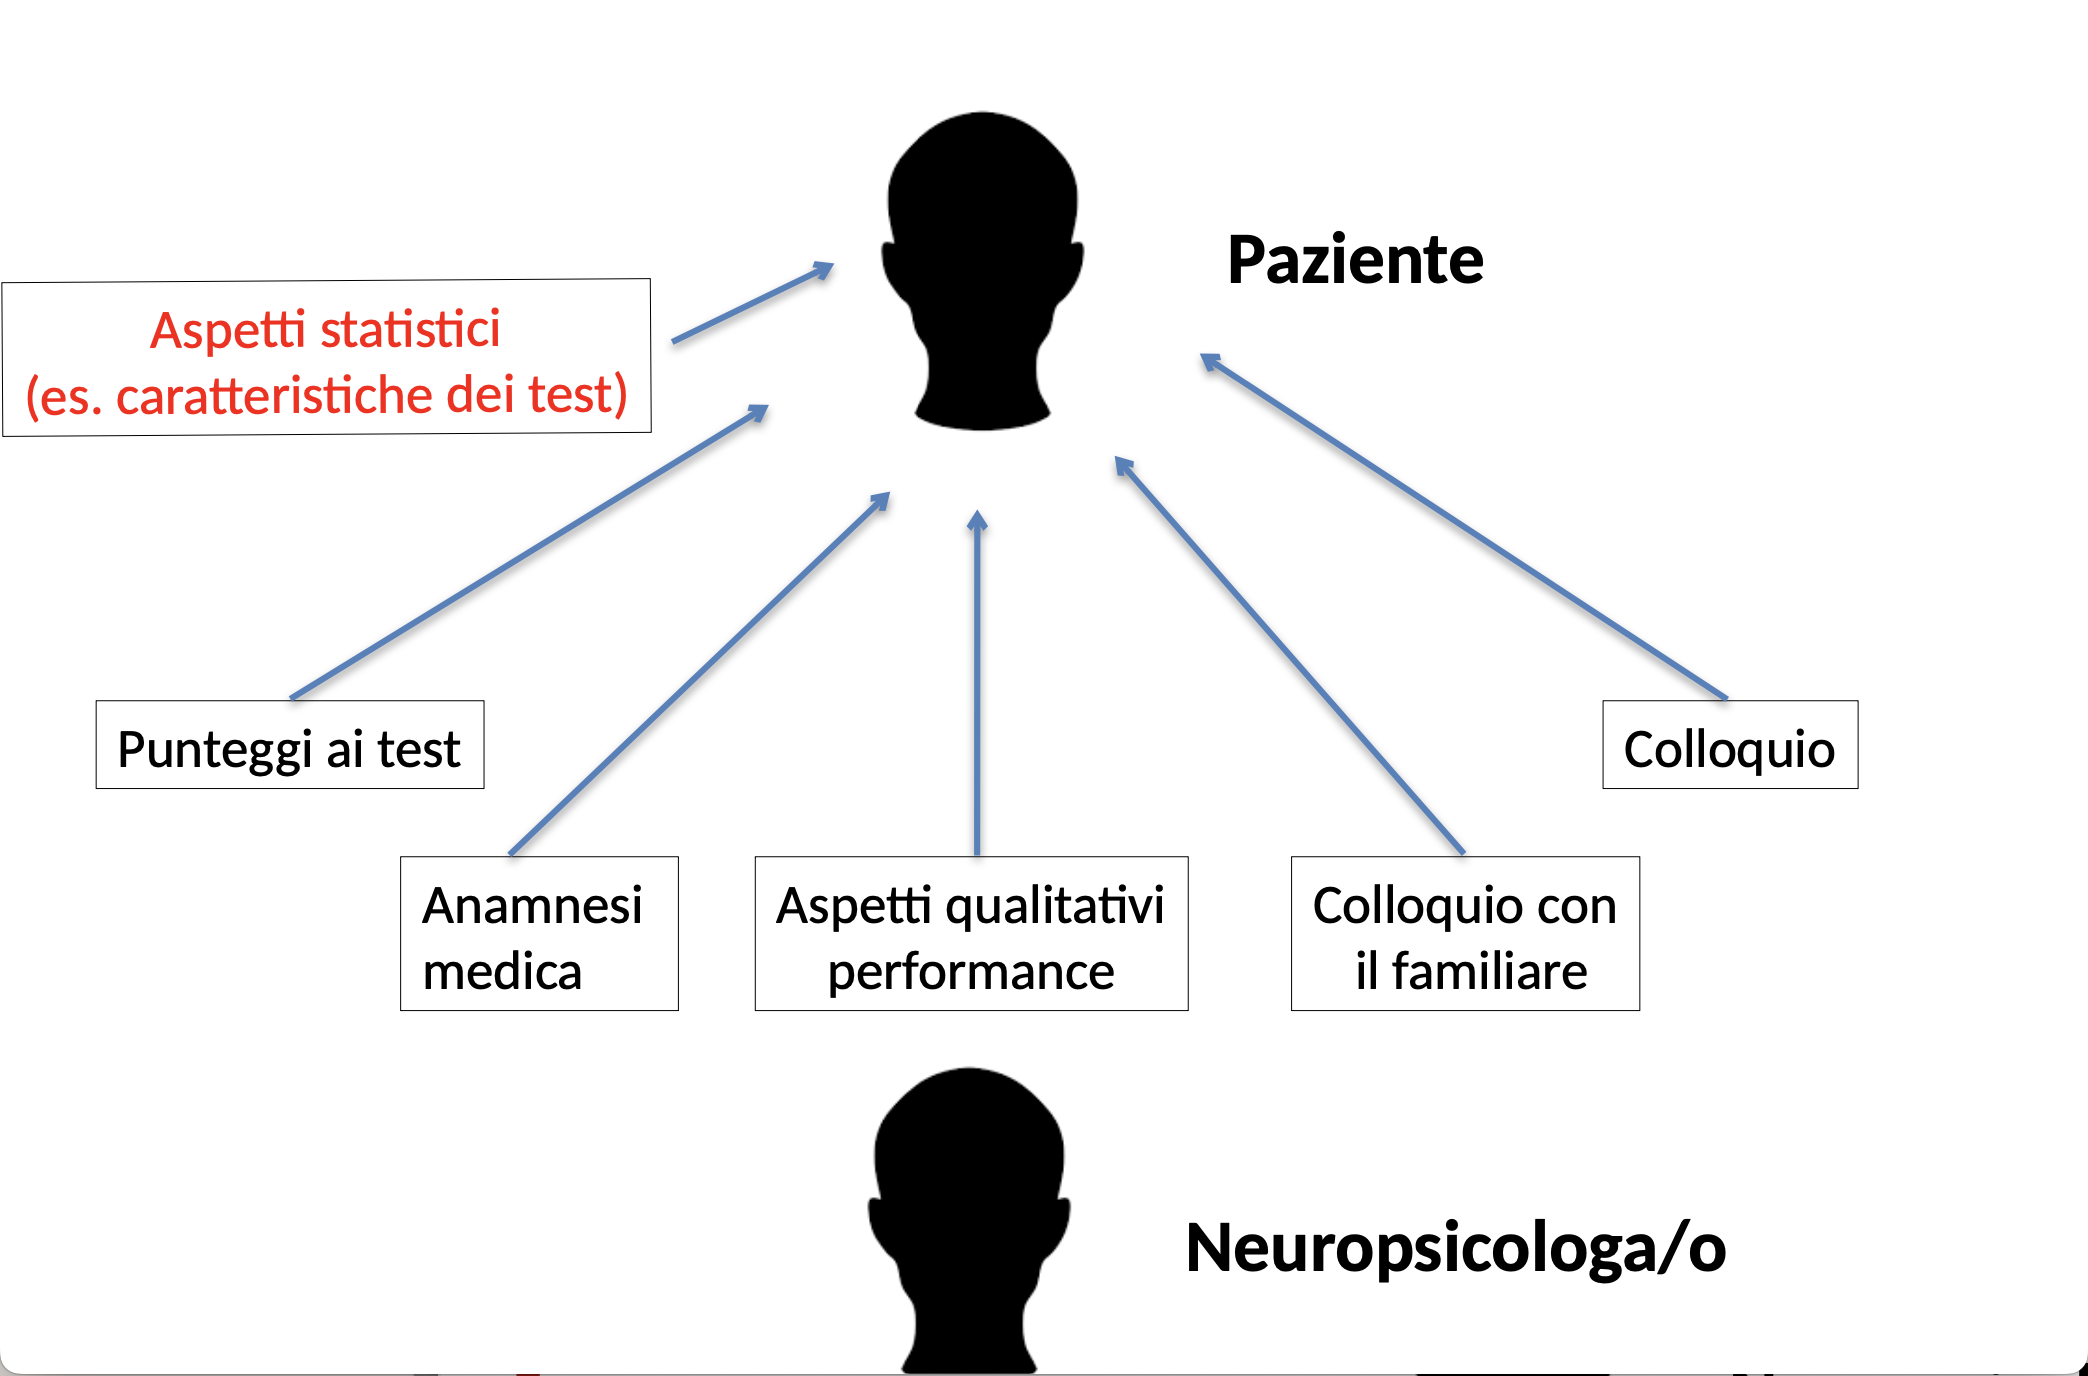
\includegraphics[keepaspectratio]{Figures/Active_collection.png}}
\end{frame}

\begin{frame}{Valutazione Neuropsicologica come raccolta di
informazioni}
\phantomsection\label{valutazione-neuropsicologica-come-raccolta-di-informazioni-1}
La raccolta di informazioni è un processo \textbf{attivo} del
neuropsicologo e dipende dalle sue conoscenze.

La stessa osservazione dipende dalle conoscenze, visto che i
comportamenti che notiamo o osserviamo \emph{(``teoreticità
dell'osservazione'')}

Così come tra queste conoscenze ci sono le conoscenze relative alle
caratteristiche dei test e alle informazioni che, realmente, possiamo
trarne.
\end{frame}

\begin{frame}{Valutazione neuropsicologica e forense}
\phantomsection\label{valutazione-neuropsicologica-e-forense}
Esistono vari obiettivi che potrebbe avere una valutazione forense,
alcuni dei quali molto complessi (es. giudicare la \emph{capacità di
intendere e volere}). In questo corso ci concentreremo su esempi sul
concetto di \textbf{danno}, ma anticipo che la definizione di danno è
diversa in ambito giuridico e in ambito clinico.
\end{frame}

\begin{frame}{Un esempio che ci accompagnerà}
\phantomsection\label{un-esempio-che-ci-accompagneruxe0}
\scriptsize

\emph{GH è un uomo di 68 anni, vedovo al centro di un contenzioso con
una compagnia di assicurazione.Al momento critico della nostra
valutazione ha appena avuto un trauma cranico in seguito ad un piccolo
incidente stradale, in cui però ha battuto la testa e perso conoscenza.
L'unico figlio sostiene che come conseguenza suo padre ha avuto un
importante peggioramento nel funzionamento cognitivo che si manifesta in
incapacità di comprendere bene ciò che gli viene detto.}

\emph{Nell'anamnesi di GH c'è però un evento rilevante. Quando era più
giovane (a 30 anni) sistemando il tetto di un garage, GH è caduto da una
scala e ha battuto la testa. Andato in ospedale non è stato
diagnosticato un trauma cranico, ma poco dopo sono accaduti una serie di
eventi: ha perso il lavoro che aveva da tempo in una piccola azienda e
ha divorziato con la moglie.}

\emph{La neuropsicologia forense entra in gioco per due motivi. I
consulenti per l'assicurazione sostengono che il problema di GH è legato
al trauma cranico subito molti anni prima e quindi non legato
all'incidente stradale. Secondo i consulenti incaricati da GH invece il
danno non è riconducibile al precedente (e non documentato) trauma, ma
solo a quello più recente.}
\end{frame}

\begin{frame}{Un esempio che ci accompagnerà (APACS)}
\phantomsection\label{un-esempio-che-ci-accompagneruxe0-apacs}
\begin{columns}
\column{0.5\textwidth}

\begin{figure}
\includegraphics[width=\textwidth]{Figures/APACS_test.png}
\end{figure}

\column{0.5\textwidth}
6 task: 2 per produzione e 4 per comprensione

\emph{(Arcara \& Bambini, 2016)}

3 punteggi globali

\end{columns}
\end{frame}

\begin{frame}{Un esempio che ci accompagnerà (Linguaggio Figurato 1)}
\phantomsection\label{un-esempio-che-ci-accompagneruxe0-linguaggio-figurato-1}
\pandocbounded{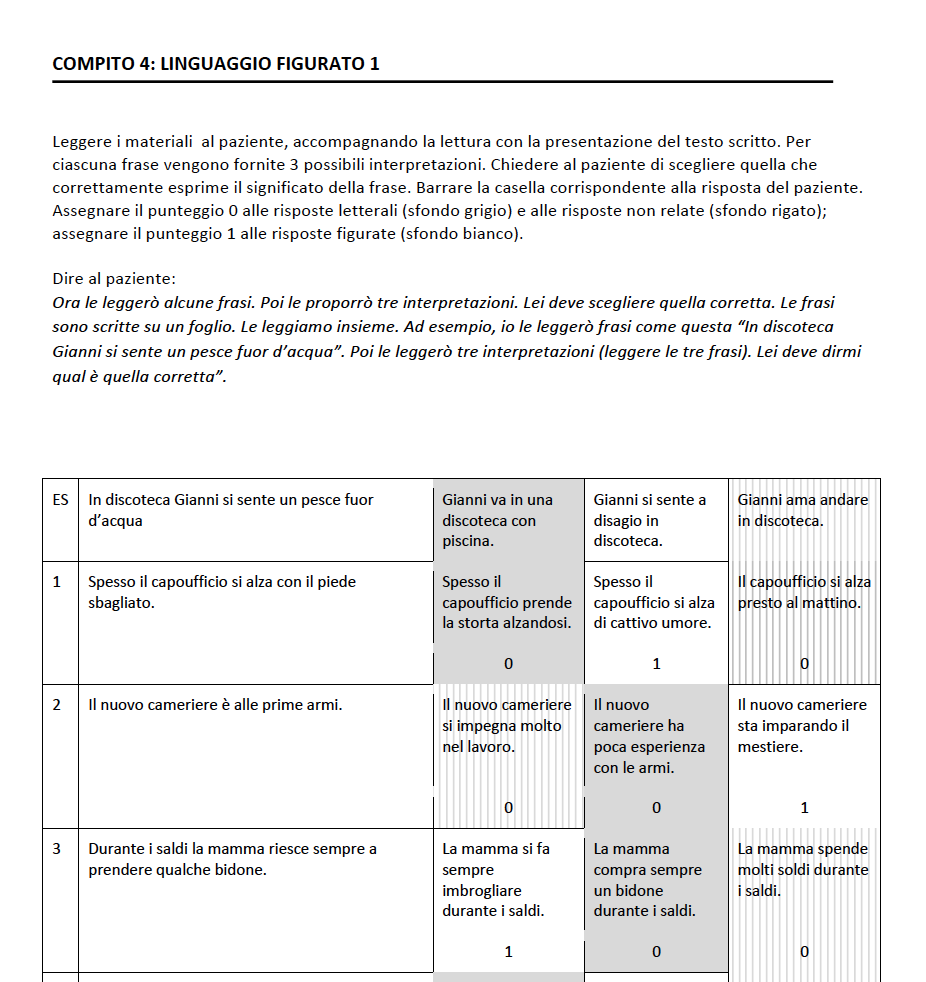
\includegraphics[keepaspectratio]{Figures/APACS_Fig_lang_1.png}}
\end{frame}




\end{document}
